\documentclass[11pt,a4paper]{article}
\usepackage[margin=25mm,headheight=14pt]{geometry}
\usepackage[T1]{fontenc}
\usepackage[utf8]{inputenc}
\usepackage{lmodern,amsmath,amssymb}
\usepackage{xcolor,graphicx,booktabs,longtable,array}
\usepackage{microtype,enumitem,fancyhdr,titlesec}
\usepackage{hyperref}
\definecolor{accent}{HTML}{163B55}
\hypersetup{colorlinks=true,linkcolor=accent,urlcolor=accent,
 pdftitle={A leading Heun root at a branch point of its limiting spectral tree},pdfauthor={Matthew J. Colbrook},
 pdfsubject={AIM 1032: mathematical result and proof}}
\urlstyle{same}
\Urlmuskip=0mu plus 1mu
\setlength{\parindent}{0pt}
\setlength{\parskip}{0.35em}
\setlength{\emergencystretch}{3em}
\setlist{itemsep=0.25em,topsep=0.3em}
\providecommand{\tightlist}{\setlength{\itemsep}{0pt}\setlength{\parskip}{0pt}}
\titleformat{\section}{\normalfont\large\bfseries\color{accent}}{\thesection}{0.7em}{}
\titleformat{\subsection}{\normalfont\normalsize\bfseries}{\thesubsection}{0.6em}{}
\pagestyle{fancy}
\fancyhf{}
\fancyhead[L]{\small\sffamily AIM 1032}
\fancyhead[R]{\small\sffamily Matthew J. Colbrook}
\fancyfoot[C]{\thepage}
\renewcommand{\headrulewidth}{0.3pt}
\setcounter{secnumdepth}{0}
\allowdisplaybreaks[2]
\title{\textbf{A leading Heun root at a branch point of its limiting spectral tree}}
\author{Matthew J. Colbrook\\[3pt]
{\small Department of Applied Mathematics and Theoretical Physics}\\
{\small University of Cambridge, United Kingdom}\\
{\small\href{mailto:mjc249@maths.cam.ac.uk}{\texttt{mjc249@maths.cam.ac.uk}}}}
\date{3 November 2026}
\begin{document}
\maketitle
\begin{abstract}
For a third-order Heun operator with leading coefficient $z^4-z$, we prove convergence of the complete sequence of Van Vleck root-counting measures to an explicit positive law supported on a three-spoke star. The leading root zero is a branch point, refuting the universal leaf assertion in AIM 1032. The proof uses total nonnegativity, compounds and moment determinacy on an interval.
\end{abstract}
\noindent\textbf{Repository target.}
This manuscript concerns AIM problem 1032 at revision
\texttt{3fa50884d129}. Its scope is stated below.
\medskip

The universal leaf assertion in Problem 1032 is false. Consider the
third-order Heun operator

\[
\mathfrak d=(z^4-z)\frac{d^3}{dz^3},\qquad Q_1=Q_2=0.
\]

Its leading coefficient has the four simple, noncollinear roots
\(0,1,\omega,\omega^2\), where \(\omega=e^{2\pi i/3}\). We prove that
the full sequence of Van Vleck root-counting measures converges to the
explicit probability law

\[
\boxed{\mu_n\Longrightarrow\operatorname{Law}(\omega^JYX^{1/3}),}
\tag{1}
\]

where the independent variables satisfy

\[
X\sim\operatorname{Beta}(1/3,2/3),\qquad
Y\sim\operatorname{Beta}(1,1/3),\qquad
\mathbb P(J=j)=\frac13\quad(j=0,1,2).
\]

The support of this limit is exactly

\[
T=[0,1]\cup\omega[0,1]\cup\omega^2[0,1].
\tag{2}
\]

Thus the leading root zero is a vertex of valency three, rather than a
leaf.

This disproves the precise universal statement in the pinned catalogue
and the same leaf clause in Shapiro--Tater (2008), Conjecture 3, and
Shapiro (2026), Conjecture 1. The example is consistent with weak
convergence, positivity, and support on a finite tree. It does not
refute a conjecture restricted to generic leading polynomials; Shapiro's
later Conjecture 2 explicitly has such a restriction.

\begin{figure}[htbp]
\centering
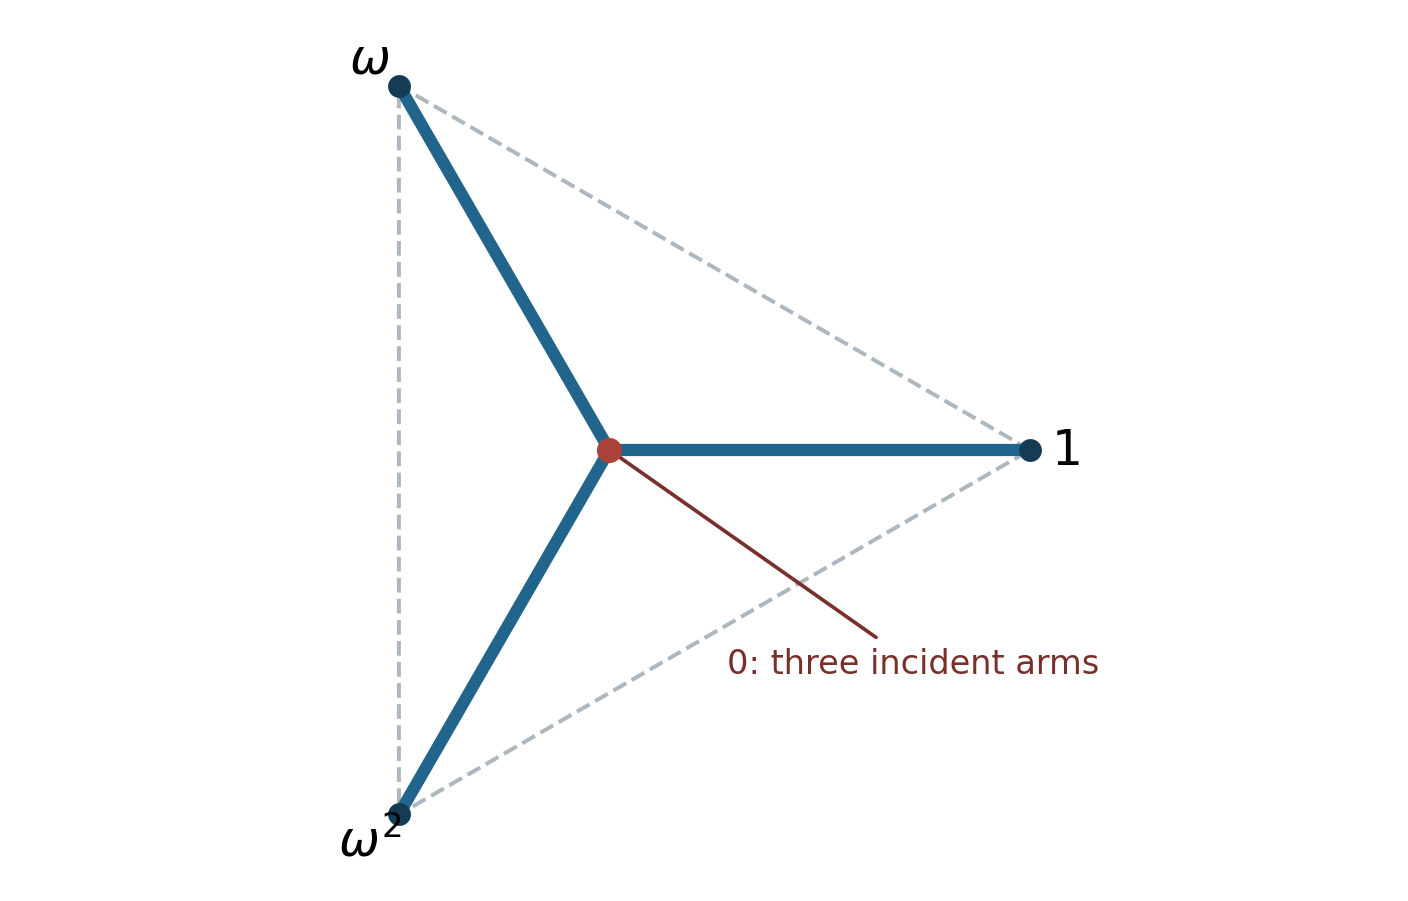
\includegraphics[width=0.68\textwidth]{figures/heun_star.png}
\caption{The exact support of the limiting root measure. The dashed
triangle is the convex hull of the leading roots; the origin is a
branch point with three incident arms.}
\end{figure}

\hypertarget{1032-van-vleck-roots-as-finite-matrix-eigenvalues}{%
\section{1. Van Vleck roots as finite-matrix
eigenvalues}\label{1032-van-vleck-roots-as-finite-matrix-eigenvalues}}

For \(n\geq3\), set \(\theta_n=n(n-1)(n-2)\) and define an operator on
polynomials of degree at most \(n\) by

\[
A_n=z-\frac{z^4-z}{\theta_n}\frac{d^3}{dz^3}.
\]

Put \(c_j=j(j-1)(j-2)/\theta_n\), with \(c_0=c_1=c_2=0\). On monomials,

\[
A_nz^j=(1-c_j)z^{j+1}+c_jz^{j-2},
\qquad 0\leq j\leq n,
\tag{3}
\]

where a term with zero coefficient is omitted. The raising term vanishes
at \(j=n\), so \(A_n\) preserves this polynomial space.

If a polynomial \(S\) of degree \(n\) solves

\[
(z^4-z)S'''+V(z)S=0,
\]

comparison of the highest-degree coefficient forces
\(V(z)=-\theta_n(z-t)\) for some \(t\). The equation is then
\(A_nS=tS\). Conversely, every eigenvector of \(A_n\) has degree \(n\):
if its highest degree were \(j<n\), the nonzero raising term
\((1-c_j)z^{j+1}\) could not be cancelled. Thus the eigenvalues of
\(A_n\), counted with algebraic multiplicity, are exactly the Van Vleck
roots in the problem.

If these roots are \(t_{n,1},\ldots,t_{n,n+1}\) with multiplicity, the
measure under discussion is

\[
\mu_n=\frac1{n+1}\sum_{j=1}^{n+1}\delta_{t_{n,j}}.
\]

The matrix in (3) is nonnegative and each column sums to one. Its
eigenvalues therefore lie in the closed unit disk. Its zeroth row
vanishes. Restriction to the invariant subspace spanned by
\(z,z^2,\ldots,z^n\) gives an \(n\times n\) matrix \(B_n\), with

\[
\det(tI-A_n)=t\det(tI-B_n).
\tag{4}
\]

\hypertarget{1032-exact-star-support-for-every-degree}{%
\section{2. Exact star support for every
degree}\label{1032-exact-star-support-for-every-degree}}

Write \(n=3q+r\), where \(r\in\{0,1,2\}\) and \(q\geq1\). Group the
monomials \(z,\ldots,z^n\) according to degrees congruent to \(1,2,0\)
modulo three, in that order. Their dimensions are

\[
d_1=q+\mathbf1_{\{r\geq1\}},\qquad
d_2=q+\mathbf1_{\{r=2\}},\qquad d_3=q.
\]

In this basis,

\[
B_n=
\begin{pmatrix}
0&0&L\\
U_1&0&0\\
0&U_2&0
\end{pmatrix},
\tag{5}
\]

where \(L\) is a \(d_1\times q\) lower bidiagonal matrix, \(U_1\) is a
\(d_2\times d_1\) upper bidiagonal matrix, and \(U_2\) is a
\(q\times d_2\) upper bidiagonal matrix. In zero-based indices, their
nonzero entries are

\[
(U_1)_{a,a}=1-c_{1+3a},\qquad
(U_1)_{a,a+1}=c_{4+3a},
\]

\[
(U_2)_{a,a}=1-c_{2+3a},\qquad
(U_2)_{a,a+1}=c_{5+3a},
\]

\[
L_{a,a}=c_{3+3a},\qquad
L_{a+1,a}=1-c_{3+3a},
\]

whenever the indicated row and column exist. All these entries are
positive. In particular, the leading \(q\times q\) blocks have positive
diagonal entries and positive first off-diagonal entries in their
indicated directions.

Consider the square return matrix on the third residue class,

\[
C_q=U_2U_1L.
\tag{6}
\]

We next prove that its eigenvalues are positive and simple.

\hypertarget{1032-total-nonnegativity-and-the-compound-argument}{%
\subsection{Total nonnegativity and the compound
argument}\label{1032-total-nonnegativity-and-the-compound-argument}}

A matrix is totally nonnegative when all minors with increasing row and
column indices are nonnegative. Each of the rectangular bidiagonal
factors in (6) has this property. Indeed, in any nonzero minor the
bidiagonal pattern permits only an order-preserving matching of row and
column indices; its determinant is therefore a product of nonnegative
entries.

For \(1\leq p\leq q\), the \(p\)-th compound matrix \(C_q^{[p]}\) has
rows and columns indexed by the \(p\)-element subsets of
\(\{0,\ldots,q-1\}\), and its entries are the corresponding minors.
Cauchy--Binet implies that every compound is nonnegative. Its diagonal
entries are positive: in both Cauchy--Binet sums, retain the same index
set in all three factors and use their positive diagonal minors.

The compound also has a positive entry whenever one occupied index is
moved by one step to an adjacent vacant position, in either direction.
For one direction, use the corresponding off-diagonal minor of \(L\) and
diagonal minors in the other factors; for the reverse direction, use an
off-diagonal minor of \(U_1\). All intermediate choices stay within the
first \(q\) indices, so the extra rows and columns in the rectangular
cases cause no difficulty.

The graph of \(p\)-element subsets under these adjacent moves is
connected. Thus every compound is irreducible with positive diagonal,
and hence primitive. Perron--Frobenius gives it a unique simple
eigenvalue of maximal modulus, which is positive. The eigenvalues of the
\(p\)-th compound are the \(p\)-fold products of eigenvalues of \(C_q\).
The compound eigenvalue identity and the Perron--Frobenius facts used
here are standard matrix theory; see, for example,
Gantmakher--Krein, Section~4, cited below.
Successively applying this fact for \(p=1,\ldots,q\) shows that the
eigenvalues of \(C_q\), in decreasing modulus order, are positive and
have strictly decreasing moduli. Its determinant is positive by the
principal-minor argument, so none is zero.

Write these eigenvalues as \(s_1,\ldots,s_q>0\). For \(t\ne0\), block
elimination in (5) gives

\[
\begin{aligned}
\det(tI_n-B_n)
&=t^{d_1+d_2}\det(tI_q-t^{-2}C_q)\\
&=t^r\det(t^3I_q-C_q).
\end{aligned}
\tag{7}
\]

The identity holds for all \(t\) because both sides are polynomials.
Therefore \(B_n\) has the three cube roots of each \(s_j\) and \(r\)
additional zero eigenvalues. Equation (4) supplies one further zero
eigenvalue for \(A_n\).

Column stochasticity of \(A_n\) implies \(0<s_j\leq1\). Consequently
every Van Vleck root lies in the star \(T\) in (2), for every
\(n\geq3\). The measure \(\mu_n\) is invariant under multiplication by
\(\omega\). Its mass at zero is \((r+1)/(n+1)\), which tends to zero.

\hypertarget{1032-limiting-moments-from-closed-paths}{%
\section{3. Limiting moments from closed
paths}\label{1032-limiting-moments-from-closed-paths}}

For a fixed nonnegative integer \(\ell\),

\[
\int z^{3\ell}\,d\mu_n(z)
=\frac1{n+1}\operatorname{tr}(A_n^{3\ell}).
\tag{8}
\]

A closed path of length \(3\ell\) in the matrix (3) must have \(2\ell\)
upward steps of size one and \(\ell\) downward steps of size two. There
are \(\binom{3\ell}{\ell}\) orderings. For a starting index farther than
\(6\ell\) from the endpoints, all these paths are permitted. Along each
such fixed-length path,

\[
c_{j+O(1)}=(j/n)^3+O(n^{-1})
\]

uniformly in the starting index \(j\). Its weight is therefore

\[
(1-(j/n)^3)^{2\ell}(j/n)^{3\ell}+O(n^{-1}).
\]

Only a bounded number of starting indices are excluded at the endpoints,
and all path weights are at most one. Taking the normalized trace and
using a Riemann sum gives

\[
\begin{aligned}
\lim_{n\to\infty}\int z^{3\ell}\,d\mu_n(z)
&=\binom{3\ell}{\ell}
  \int_0^1(1-t^3)^{2\ell}t^{3\ell}\,dt\\
&=\frac{\Gamma(3\ell+1)\Gamma(\ell+1/3)}
 {3\,\Gamma(\ell+1)\Gamma(3\ell+4/3)}
=:m_\ell.
\end{aligned}
\tag{9}
\]

The same closed-path argument gives zero for every holomorphic moment
whose order is not divisible by three. Formula (9) gives \(m_0=1\).

The exact support result from Section 2 is essential here. Holomorphic
moments alone would not determine an arbitrary measure inside a
two-dimensional convex hull.

\hypertarget{1032-identification-of-the-probability-law-and-its-full-support}{%
\section{4. Identification of the probability law and its full
support}\label{1032-identification-of-the-probability-law-and-its-full-support}}

Let \(\rho_n\) be the pushforward of \(\mu_n\) under \(z\mapsto z^3\).
By Section 2, \(\rho_n\) is a probability measure on \([0,1]\). Equation
(9) gives the limit of every ordinary moment.

For the independent beta variables in (1), the beta integral gives

\[
\mathbb E[X^\ell]
=\frac{\Gamma(\ell+1/3)}
 {\Gamma(1/3)\Gamma(\ell+1)},
\]

\[
\mathbb E[Y^{3\ell}]
=\frac{\Gamma(3\ell+1)\Gamma(4/3)}
 {\Gamma(3\ell+4/3)}.
\]

Since \(\Gamma(4/3)=\Gamma(1/3)/3\), their product is exactly
\(m_\ell\). Polynomials are dense in \(C([0,1])\), so convergence of
these moments proves

\[
\rho_n\Longrightarrow\operatorname{Law}(XY^3).
\tag{10}
\]

Both beta densities are positive on \((0,1)\). Their product variable
\(XY^3\) therefore has support all of \([0,1]\).

Rotation invariance determines \(\mu_n\) from \(\rho_n\). For every
continuous function \(f\) on \(T\),

\[
\int_T f(z)\,d\mu_n(z)
=\int_0^1\frac13\sum_{j=0}^2
 f(\omega^j s^{1/3})\,d\rho_n(s).
\]

The function on the right is continuous also at zero. Taking the limit
in (10) proves (1), and its support is exactly the three-spoke star
\(T\).

\hypertarget{1032-contradiction-to-the-universal-leaf-clause}{%
\section{5. Contradiction to the universal leaf
clause}\label{1032-contradiction-to-the-universal-leaf-clause}}

The roots of \(Q_3(z)=z^4-z\) are simple: \(Q_3'(0)=-1\), while \(Q_3'\)
equals \(3\) at each nonzero root. They are not all collinear. Thus the
operator meets all the stated hypotheses.

Nevertheless, the support of its limiting measure contains three
nontrivial arms issuing from zero. Zero has valency three and cannot be
a leaf. This also contradicts the weaker interpretation that the measure
need only be supported on some larger finite tree: any such closed tree
contains the support \(T\), and zero cannot become a leaf when a set
containing these three arms is enlarged to another tree. Connecting two
of the arms elsewhere would instead create a cycle.

A corrected statement must allow some leading roots to be internal
vertices or impose an additional restriction that excludes this example.
The proof supplies the actual positive limit and its full support; the
counterexample is not based only on exterior moments or a numerical root
plot.

\hypertarget{1032-a-higher-order-family}{%
\section{6. A higher-order family}\label{1032-a-higher-order-family}}

The same argument, along degrees \(n=kq\), applies to

\[
\mathfrak d=(z^{k+1}-z)D^k,\qquad k\geq3.
\]

The limit is the law of \(\omega_k^JYX^{1/k}\), where

\[
\omega_k=e^{2\pi i/k},\qquad
X\sim\operatorname{Beta}(1/k,1-1/k),\qquad
Y\sim\operatorname{Beta}(1,1/k),
\]

and \(J\) is independently uniform on \(\{0,\ldots,k-1\}\). Its support
is the \(k\)-spoke star, with zero a leading root of valency \(k\). The
fully proved third-order case already suffices to disprove the universal
claim.

\hypertarget{1032-references-and-verification-scope}{%
\section{References and verification
scope}\label{1032-references-and-verification-scope}}

\begin{enumerate}
\def\labelenumi{\arabic{enumi}.}
\tightlist
\item
  B. Shapiro and M. Tater, \emph{On spectral polynomials of the Heun
  equation. I}, arXiv:0812.2321 (2008), Section 4, Conjecture 3, printed
  p.~13. \url{https://arxiv.org/pdf/0812.2321}.
\item
  B. Shapiro, \emph{Van Vleck spectra of high-order Heun operators:
  finite-band universality and exterior asymptotics}, arXiv:2607.02700
  (2026), Conjecture 1, printed p.~4. The later Conjecture 2 explicitly
  assumes genericity and is not refuted here.
  \url{https://arxiv.org/pdf/2607.02700}.
\item
  F. Gantmakher and M. Krein,
  \emph{Sur les matrices complètement non négatives et oscillatoires},
  Compositio Mathematica \textbf{4} (1937), 445--476.
  Section~4, p.~461, states the compound eigenvalue-products identity
  and the oscillatory positive-simple-spectrum theorem.
  \url{https://www.numdam.org/item/CM_1937__4__445_0.pdf}.
  The particular factorization and compound irreducibility argument are
  proved above.
\end{enumerate}

Small finite-matrix calculations were used only as checks.
Floating-point eigensolvers become unreliable for the highly nonnormal
bidiagonal products at larger degrees; the exact compound argument
proves the spectral location. No bibliographic-priority claim is made.
\end{document}
